\section{模型求解}
以学生常去的地区为区分,分别利用已知数据进行求解。使用EXCLE-solver。 由于‘可变单元格过多’,所以先将三类区域运输分配分别求值,再进行整合。\\
\indent 以300为电动自行车运输总数,进行后续计算。
\subsection{分区域-充电桩设置}
\begin{figure}[H]
    \centering
    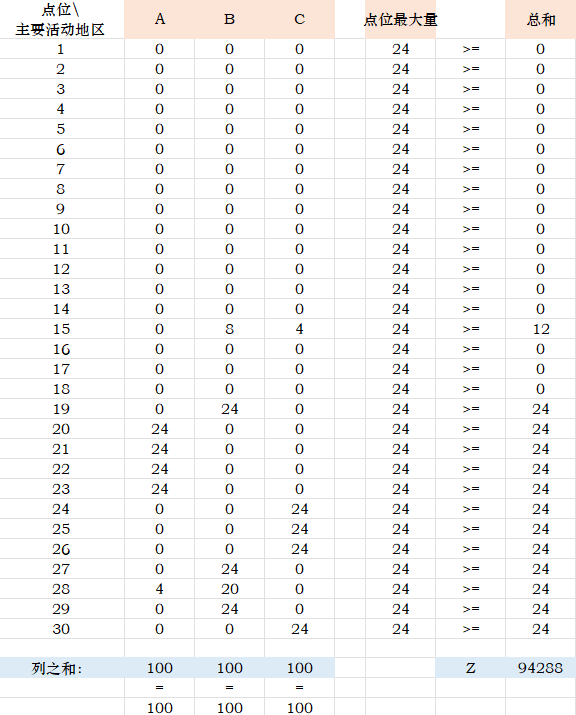
\includegraphics[width=0.5\textwidth]{pic.png}
    %\caption{自卸车卸货的两个过程}
    \caption{宿舍区-充电桩设置}
\end{figure}
\begin{figure}[H]
    \centering
    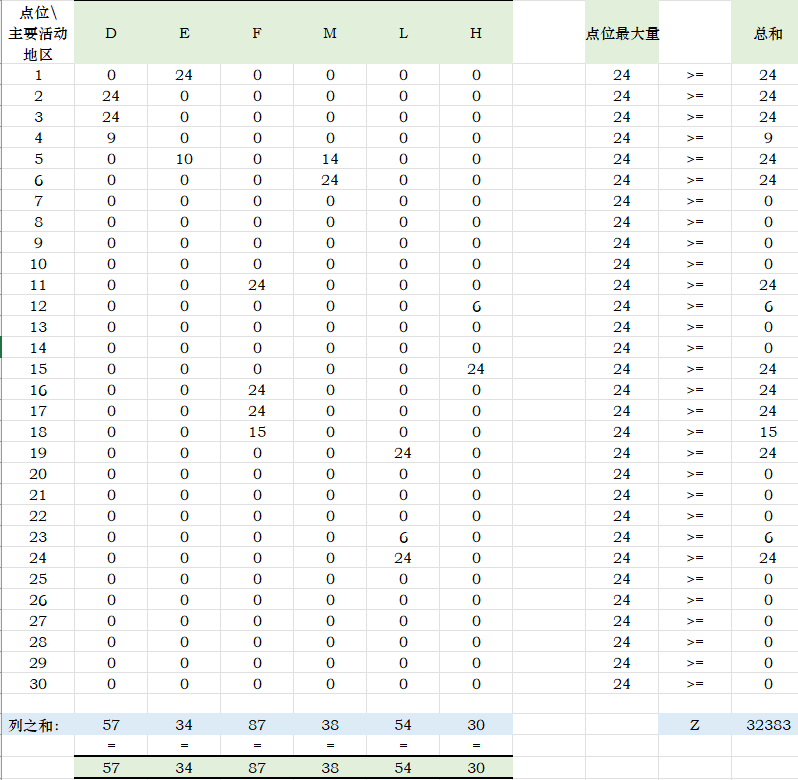
\includegraphics[width=0.5\textwidth]{pic5.png}
    %\caption{自卸车卸货的两个过程}
    \caption{学习区-充电桩设置}
\end{figure}
\begin{figure}[H]
    \centering
    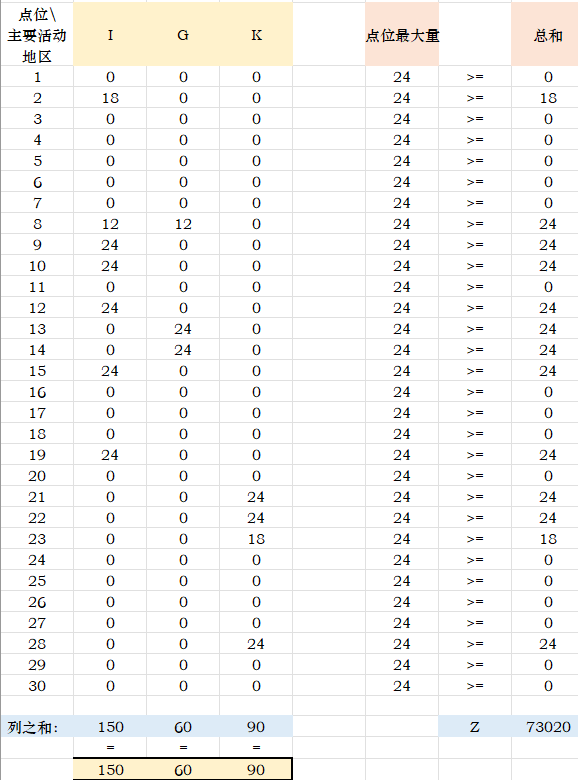
\includegraphics[width=0.4\textwidth]{pic6.png}
    %\caption{自卸车卸货的两个过程}
    \caption{其他休闲区-充电桩设置}
\end{figure}
\subsection{求解数据合并}
\begin{table}[H]
    \centering
	\caption{求解各目的地$i$可容纳电动车数目}
    \begin{tabular}{cp{3cm}<{\centering}||cp{3cm}<{\centering}||cp{3cm}<{\centering}}
        \toprule  %添加表格头部粗线
        目的地$j$ & 所需充电口数目 &  目的地$j$&所需充电口数目 & 目的地$j$&所需充电口数目\\
        \midrule  %添加表格中横线
        1 & 14  & 11 & 14 & 21 & 10 \\ 
        2 & 16  & 12 & 6  & 22 & 10 \\ 
        3 & 14  & 13 & 2  & 23 & 13 \\ 
        4 & 5  & 14 & 2  & 24 & 22 \\ 
        5 & 14  & 15 & 20  & 25 & 7 \\ 
        6 & 14  & 16 & 14  & 26 & 7 \\ 
        7 & 0  & 17 & 14  & 27 & 7 \\ 
        8 & 2  & 18 & 9  & 28 & 10 \\ 
        9 & 2  & 19 & 24  & 29 & 7 \\ 
        10 & 2  & 20 & 7  & 30 & 7 \\ 
        \bottomrule %添加表格底部粗线
    \end{tabular}
\end{table}
\begin{table}[H]
    \centering
	\caption{\textbf{排序后}求解各目的地$i$可容纳电动车数目}
    \begin{tabular}{cp{3cm}<{\centering}||cp{3cm}<{\centering}||cp{3cm}<{\centering}}
        \toprule  %添加表格头部粗线
        目的地$j$ & 所需充电口数目 &  目的地$j$&所需充电口数目 & 目的地$j$&所需充电口数目\\
        \midrule  %添加表格中横线
        19 & 24 & 17 & 14  & 29 & 7 \\ 
        24 & 22  & 23 & 13  & 30 & 7 \\ 
        15 & 20  & 21 & 10  & 12 & 6 \\ 
        2 & 16  & 22 & 10  & 4 & 5 \\ 
        1 & 14  & 28 & 10  & 8 & 2 \\ 
        3 & 14  & 18 & 9  & 9 & 2 \\ 
        5 & 14  & 20 & 7  & 10 & 2 \\ 
        6 & 14  & 25 & 7 &  13 & 2 \\ 
        11 & 14  & 26 & 7 &  14 & 2 \\ 
        16 & 14  & 27 & 7 &  7 & 0 \\ 
        \bottomrule %添加表格底部粗线
    \end{tabular}
\end{table}
